% DEVELOPMENT RUN --- not reportable; never include in the thesis.
% Generated by tools/pipeline/figures.py from a1_dryrun_20261009/metrics.json (sha256 9f27c701b18927a13a766588b5e230e6609dee023309588e844db05c92475d5a). Do not edit by hand.
\begin{figure}[htbp]
\centering
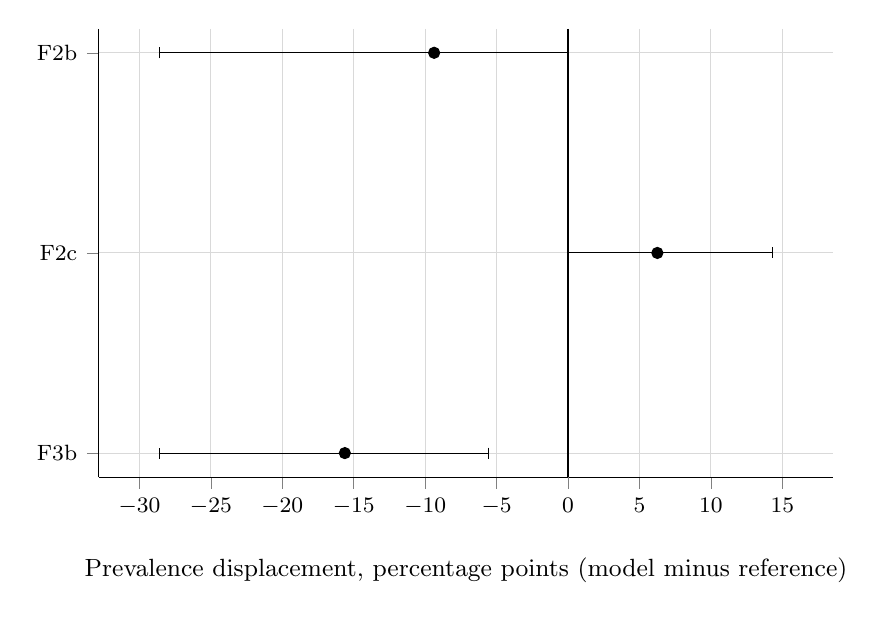
\begin{tikzpicture}
\begin{axis}[
  width=0.9\textwidth, height=0.6\textwidth,
  xlabel={Prevalence displacement, percentage points (model minus reference)}, xlabel style={font=\small},
  symbolic y coords={F2b,F2c,F3b}, ytick=data, y dir=reverse,
  yticklabel style={font=\footnotesize}, xticklabel style={font=\footnotesize},
  axis lines*=left, tick align=outside, enlarge y limits=0.06, grid=major, grid style={black!15},
  extra x ticks={0}, extra x tick labels={}, extra x tick style={grid=major, grid style={black, thick}},
]
\addplot[only marks, mark=*, mark options={fill=black}, error bars/.cd, x dir=both, x explicit] coordinates {(-9.375,F2b) -= (19.196,0) += (9.375,0) (6.250,F2c) -= (6.250,0) += (8.036,0) (-15.625,F3b) -= (12.946,0) += (10.069,0)};
\end{axis}
\end{tikzpicture}
\caption{\textbf{DEVELOPMENT RUN --- not reportable.} Design-weighted, reference-relative prevalence displacement per frame element in the pooled population: the share of paragraphs on which the model marks the element minus the share on which the reference does, in percentage points of the eligible frame. Bars are the 2.5--97.5 percentile interval over 2000 article resamples; no bias-correction estimator is applied; opposing errors can cancel, and the interval carries no uncertainty from the human reference. Elements with fewer than $s=5$ reference paragraphs are not plotted; table~5 prints their state. Run \texttt{a1\_dryrun\_20261009}.}
\label{fig:displacement_pooled}
\end{figure}
